% !TeX root = ../main.tex
% Add the above to each chapter to make compiling the PDF easier in some editors.

\chapter{Theoretical Foundations}\label{chapter:theoreticalFoundacions}

In this chapter, we investigate the theoretical foundations by examining database performance measurements and in the next step describing used datasets and the data structure.\\We will start by discussing the characterisitcs of database systems and elaborate on the significance of performance measurements in this context. Additionally, we will outline the common performance metrics, that play a central role in the evaluation of performance analysis.
\\ For clarifying used datasets and the data structure, we commence by describing the utilized performance data, followed by giving an overview of the structure of the Benchy Viewer's input file containing the performance measurements. Moreover, the data prepration for this input file will be explained.

\section{Database Systems and Performance Measurements}
Performance measurement and analysis are fundamental in the realm of database systems. They offer valuable insights into system behavior, helping to pinpoint bottlenecks and optimization opportunities. This process is crucial not only for evaluating one's own system but also for making meaningful comparisons with other systems. Visualisations play a pivotal role in understanding performance data and are often used to convey complex findings effectively.
To interpret performance data effectively, we begin by understanding the characteristics and core traits of a Database System.

\subsection{Characteristics of Database Systems}
Database systems are complex structures that manage and store vast amounts of data efficiently, involving interrelated factors that must be finely tuned to ensure optimal performance.\\
One of the fundamental functions of a database system is query processing. A query is essentially a request for specific information from the database. This involves receiving and then executing that query. The process includes tasks like parsing, optimization, and execution.\\
Queries go through two main phases: compilation and execution. \textcolor{red}{Figure mit Compilation und Execution} During compilation, the query is transformed into an execution plan. This plan outlines the steps the system should take to retrieve the requested data. In the execution phase, the system follows this plan to fetch the data.\\
Query plans are roadmaps that guide how a database executes queries, with operators as specialized components responsible for specific actions. Operators, like selection and join operators, perform data operations during query execution, such as filtering and combining data. Optimizing query plans is vital for database efficiency, with query optimizers selecting the best plan considering factors like data distribution and hardware capabilities.\\
Query processing can be time-consuming due to various challenges. For instance, complex queries, large datasets, and suboptimal query plans can lead to slow performance. Identifying and overcoming these challenges is essential for improving system efficiency.

Understanding these characteristics is key to understanding the complexity of database performance. Challenges such as optimising query plans and dealing with large data sets are common, and manual assessment is often impractical.\\
The need for objective metrics is therefore obvious, making performance measurements essential for targeted optimisations. Due to the complexity of these metrics, visualisation techniques are invaluable for easier interpretation and analysis.\\
In the next section, we will explore the important role of performance measurements and their visualisation in improving database efficiency.


\subsection{Importance of Performance Measurements}
Database systems are the core of a wide range of applications. Consequently, their performance matters not just in terms of user-friendliness and reliability, but also in terms of efficiency. Performance measurements play a central role in this context.\\
One of the key advantages of performance measurements lies in their capacity to assist in optimization efforts. By quantifying performance in a series of metrics, database developers can pinpoint precisely where bottlenecks occur, whether it is in the compilation phase, the query plan, data retrieval, or any other component of the database system. This focused approach minimizes the trial and error often involved in performance tuning and directs resources toward the most impactful modifications.\\
Furthermore, bottlenecks and areas with room for improvement are often not obvious. With the aid of performance measurements, these elements come into sharp focus. Measurements can reveal, for example, if the system's weak point lies in query compilation or if the query plan needs to be optimized. Understanding and interpreting the findings correctly is crucial for making informed decisions on where to prioritize improvement efforts.\\
Another fundamental aspect is scalability. In a world where data is continuously growing, the scalability of a database system becomes a certain priority, because data volumes continue to grow. Performance measurements can identify the limitations of a system as it scales, revealing performance degradation points before they become critical bottlenecks. This approach is not only applied to solve current needs of data volume, but is also contributing to the system's scalability for the future.\\
Referring back to the introduction's implication, the complexity of performance metrics can often be overwhelming. Visualisation techniques become invaluable tools in this context. By translating numerical data into graphical elements, these visualisations can illuminate patterns and trends that could otherwise be easily overlooked, offering an intuitive and interactive way to understand the performance bottlenecks and operational nuances.

In summary, performance measurements are essential in the effective management and optimization of complex database systems. With these basic principles in mind, the next section examines common performance metrics for evaluating database systems, which serve as the quantitative backbone for the analyses and visualisations discussed here.

\subsection{Common Performance Metrics}
Understanding the importance of performance measurements in database systems necessitates a deeper dive into the specific metrics that help analyse various aspects of performance. This section explores effective metrics and how they are used within this domain, which indicates the desired functionalities of the Benchy Viewer in terms of interaction and visualisation.\\
In the paper "Bringing Compiling Databases to RISC Architectures" \cite{Bringin-Compiling-Databases-to-RISC} the compilation performance of the dominant x86-64 server architecture is contrasted  with the new introduced code generator designed for AArch64-based systems. This is interesting for the Benchy Viewer as it conducts a comparative analysis of different perspectives in terms of performance,  leveraging specific performance metrics that are also visually represented.\\ 
The paper utilizes both quantitative and subjective performance metrics when addressing the query compilation strategy. However, for the scope of our visualisation, we focus on the quantitative metrics. Relying on quantitative metrics allows for clear, objective visualisation that can represent performance differences, whereas subjective metrics does not offer the same level of clarity and consistency in a visual representation.\\
Here one of the most central metrics is the throughput, a key metric in databases, measures the number of processed tuples per second and is a primary optimization target. In the context of compiling databases, throughput is primarily influenced by the quality of the generated machine code for queries.\\
Another fundamental metric is the latency, which is the time needed for generating and compiling query code before execution, with lower latency being particularly important for real-time transactional systems.\\
With these two metrics, the paper shows an intuitive and clear overview of how different database instances perform on the TPC-H benchmark, as demonstrated in Figure~\ref{fig:risc-metrics}.

\begin{figure}[h]
  \centering
  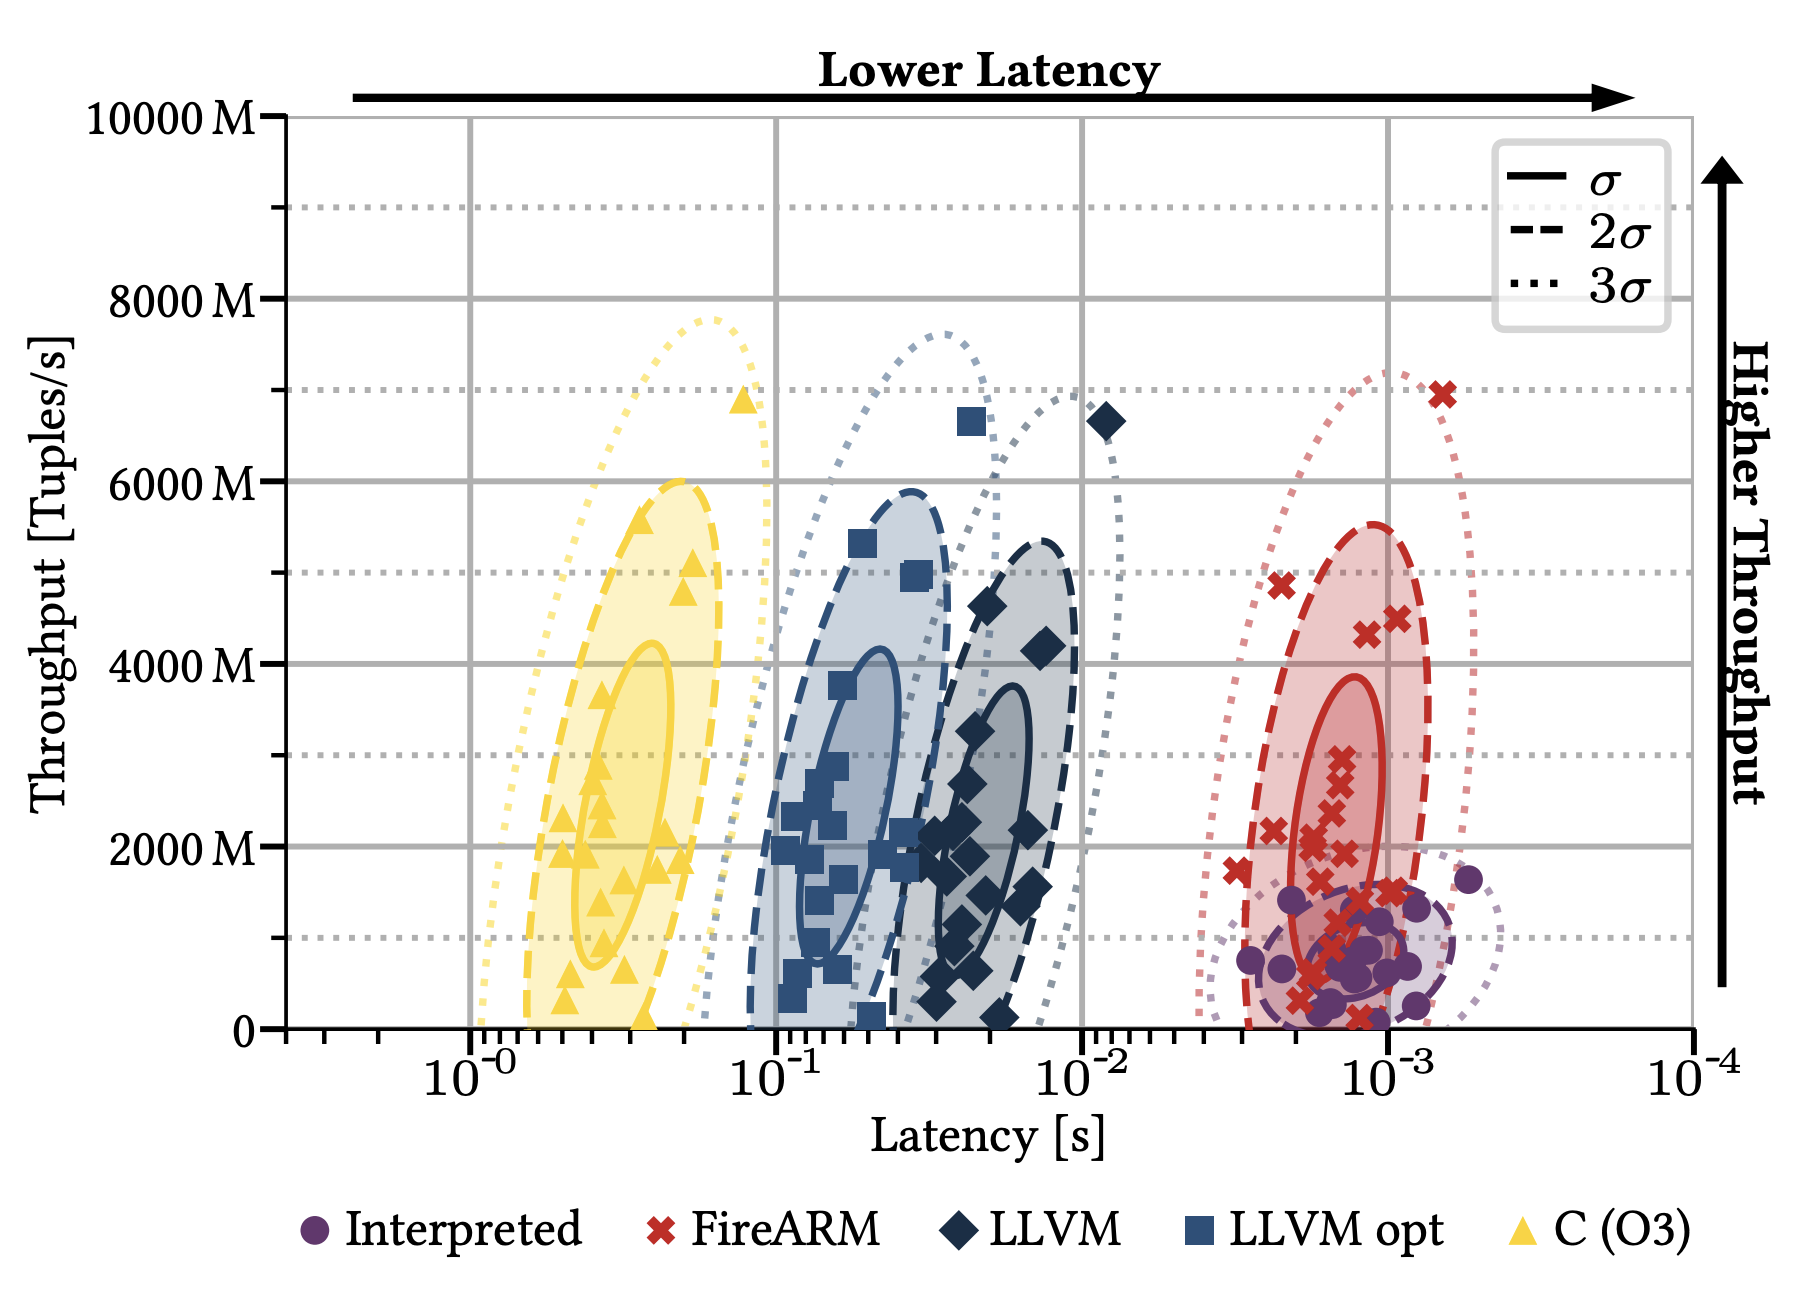
\includegraphics[width=0.8\linewidth]{figures/risc-metrcis-visualization.png}
  \caption{Visualisation example of compile-time and throughput of different query-compilation strategies running the TPC-H benchmark \cite{Bringin-Compiling-Databases-to-RISC}.}
  \label{fig:risc-metrics}
\end{figure}

\noindent

The visualisation presents a scatter plot that groups query results into clusters, with each cluster representing a database instance by a distinct color. The Y-axis displays the throughput in tuples per second, while the X-axis shows the latency in seconds, which is a descending value from left to right. Additionally, arrowed labels point to the preferred values: higher values on the Y-axis and lower on the X-axis. Thus, top-right-corner values represent optimal performance, allowing viewers to quickly identify well-performing database instances as well as the performance differences between instances.\\
In this illustration, the system highlighted in red is notable for its low latency and high throughput. Conversely, the system marked in yellow has the poorest latency performance. The instance in purple also stands out, boasting the lowest latency, but it lags behind in terms of throughput.

In the context of performance metrics, the Benchy Viewer should be capable of visualizing the key differences between instances in an intuitive and effective way. 

Besides grouping the query results into clusters, with each cluster representing a database instance, it would also be beneficial to have the flexibility to choose a specific metric for this categorization. For instance, if a database developer is primarily concerned with the metrics of execution time and throughput, they should have the option to shape the data visualisation based on these metrics.

Up next, we'll explore the dataset that is consumed by the Benchy Viewer to offer all the data and performance metrics within the analytical visualisations. We'll detail the data structure and how the data is prepared to get in this shape.

\section{Used Datasets and Data Structure}
\subsection{Description of the Utilized Performance Data}
\subsection{Structure of the CSV File with Performance Measurements}
\subsection{Data Preparation}


